%!TEX root = <main.tex>
\section{Experimental Evaluation}
We empirically validate if \system~ is able reduce the runtime taken for occlusion based deep CNN explainability workloads.
We then conduct controlled experiments to show the individual contribution of each optimization in \system~ for the overall system efficiency.

\vspace{2mm}
\noindent \textbf{Datasets.}
We use three real-world datasets: \textit{OCT}, \textit{Chest X-Ray}, and a sample from \textit{ImageNet}. \textit{OCT} has about 84,000 optical coherence tomography retinal images categorized into four categories: CNV, DME, DRUSEN, and NORMAL. CNV (choroidal neovascularization), DME (diabetic macular edema), and DRUSEN are three different varieties of Diabetic Retinopathy. NORMAL corresponds to healthy retinal images. \textit{Chest X-Ray} has about 6,000 X-ray images categorized into three categories: VIRAL, BACTERIAL, and NORMAL.
VIRAL and BACTERIAL categories corresponds to two varieties of Pneumonia. NORMAL corresponds to chest X-Rays of healthy people. Both \textit{OCT} and \textit{Chest X-Ray} datasets are obtained from an original scientific study \cite{kermany2018identifying} which uses CNNs for predicting Diabetic Retinopathy and Pneumonia from radiological images. \textit{ImageNet} sample dataset contains 1,000 images corresponding to two hundred categories selected from the original thousand categorical dataset \cite{deng2009imagenet}.

\vspace{2mm}
\noindent \textbf{Workloads.}
We use three popular ImageNet-trained deep CNNs: VGG16 \cite{vggnet}, ResNet18 \cite{resnet}, and Inception3 \cite{inception}, obtained from \cite{torchvisionmodels}. They complement each other in terms of model size, computational cost, amount of theoretical redundancy that exist for occlusion experiments, and the level of architectural complexity of the CNN model. For \textit{OCT} and \textit{Chest X-Ray} datasets, the three CNN models are fine-tuned by retraining the final fully-connected layer with hyper-parameter tuning as per standard practice. More details on the fine-tuning process are included in the Appendix. Heat map for the predicted probabilities is generated using Python Matplotlib library's \texttt{imshow} method using the \texttt{jet\_r} color scheme. For the heatmap, maximum threshold value is set to \texttt{min}$(1, 1.25 \times p)$ and minimum threshold value set to $0.75 \times p$ where $p$ is predicted class probability for the unmodified image. Original images were resized to the size required by the CNNs ($224\times224$ for VGG16 and ResNet18 and $299\times299$ for Inception3) and no additional pre-processing is done. For GPU experiments a batch size of 128 and for CPU experiments a batch size 16 is used. CPU experiments are executed with a thread parallelism of 8.
All of our datasets, fine-tuning, experiment, and system code will be made available on our project web page.

\vspace{2mm}
\noindent \textbf{Experimental Setup.}
We use a workstation which has 32 GB RAM, Intel i7-6700 @ 3.40GHz CPU, 1 TB Seagate ST1000DM010-2EP1, and Nvidia Titan X (Pascal) 12 GB memory GPU.
The system runs Ubuntu 16.04 operating system with PyTorch version of 0.4.0, CUDA version of 9.0, and cuDNN version of 7.1.2.
Each runtime reported is the average of three runs with 95\% confidence intervals.

\subsection{End-to-End Evaluation}

\begin{figure*}[t]
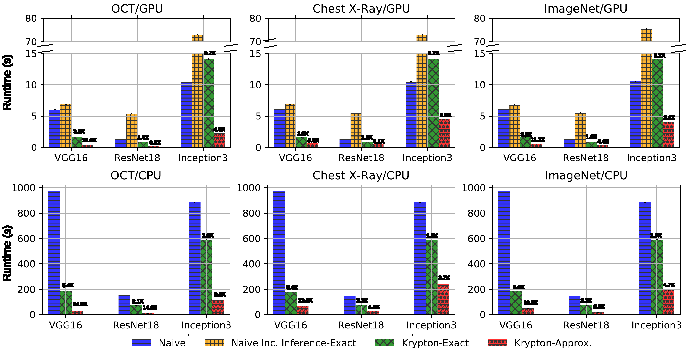
\includegraphics[width=\textwidth]{images/5_1_all_edited}
\caption{End-to-end efficiency achieved by \system~ over naive approaches.}
\label{fig:5_1_all_edited}
\end{figure*}

For the GPU based environment, we compare two variations \system~, \system-Exact which only applies the \textit{incremental inference} optimization and \system-Approximate which applies both \textit{incremental inference} and \textit{approximate inference} optimizations, against two baselines.
\textit{Naive} is the current dominant practice of performing full inference for multiple images corresponding to individual occlusion patch positions in batched manner.
\textit{Naive Incremental Inference-Exact} is a pure PyTorch based implementation of Algorithm \ref{alg:incinference} which does not use any GPU optimized kernels for memory copying where as \system~ does.
For CPU based environments we only compare \system-Exact and \system-Approximate against \textit{Naive} as no customization is needed for the pure PyTorch based implementation.
For different datasets we set \textit{adaptive drill-down} system tuning parameters differently.
For \textit{OCT} images the region of interest is relative small and hence a $r_{drill-down}$ value of 0.1 and a target \texttt{speedup} of 5 is used.
For \textit{Chest X-Ray} images the region of interest can be large and hence a $r_{drill-down}$ value of 0.4 and a target \texttt{speedup} of 2 is used.
For \textit{ImageNet} experiments we use a $r_{drill-down}$ value of $0.25$ and a target \texttt{speedup} value of 3, which are also the \system~ default values.
For all experiments, $\tau$ is configured using a separate tuning image dataset $(n=30)$ for a target SSIM of $0.9$.
Figure \ref{fig:5_1_all_edited} presents the results.

We see that \system~ improves the efficiency of the occlusion based explainability workload across the board.
...
Overall \system~ offers the best (or near-best) efficiency on these workloads.
This confirms the benefits of different optimizations performed by our system for improving the efficiency of the workload and there by to reduce the computational and runtime costs.
It also makes occlusion experiments more amenable for the interactive diagnosis of CNN predictions.



\subsection{Lesion Study}

\vspace{2mm}
\noindent \textbf{Speedups from Incremental Inference.}
\begin{figure}[t]
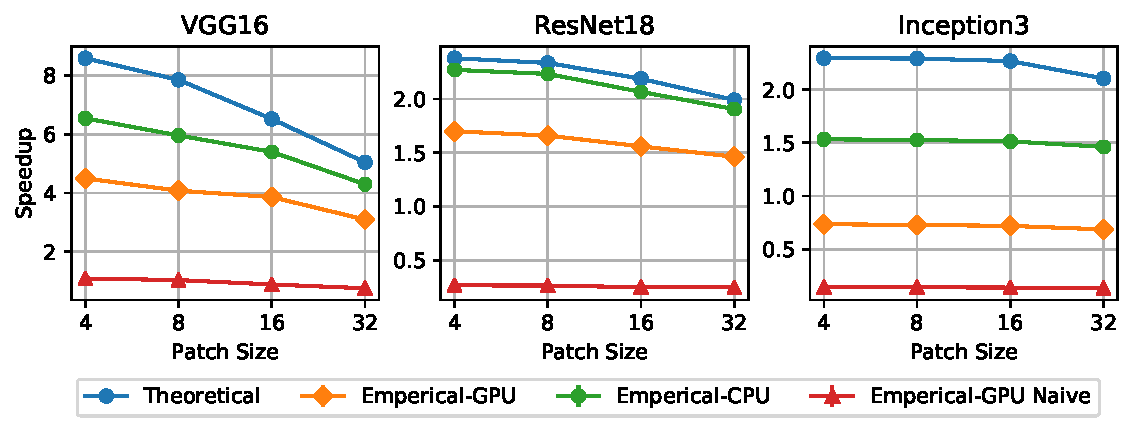
\includegraphics[width=\columnwidth]{images/5_2_1_edited}
\caption{Theoretical versus empirical speedup for \textit{incremental inference} with varying occlusion patch sizes and different CNN models (Occlusion patch stride $S=4$).}
\label{fig:5_2_1_edited}
\end{figure}

\vspace{2mm}
\noindent \textbf{Speedups from Projective Field Thresholding.}
\begin{figure}[t]
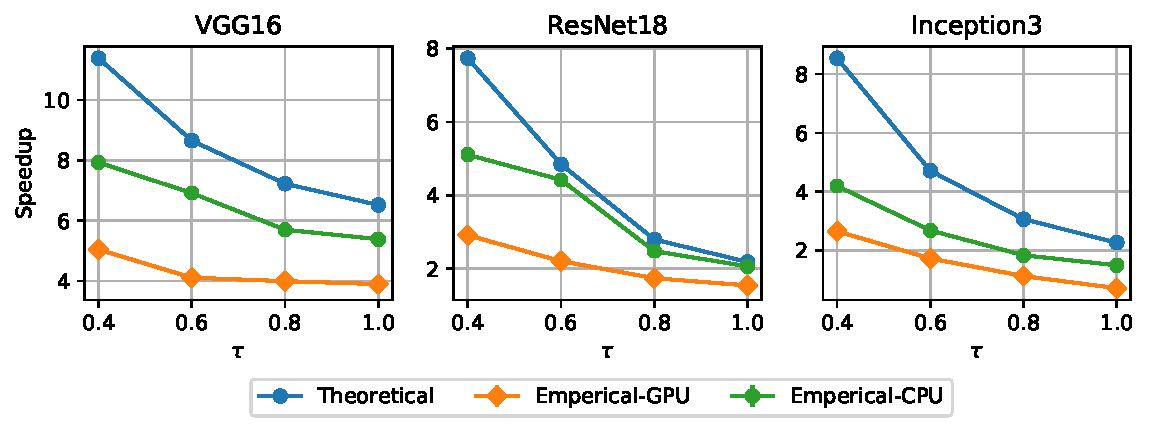
\includegraphics[width=\columnwidth]{images/5_2_2_edited}
\caption{Theoretical versus empirical speedup for \textit{incremental inference} with \textit{projective field thresholding} with varying threshold values ($\tau$) and different CNN models (Occlusion patch size = $16 \times 16$, stride $S=4$).}
\label{fig:5_2_1_edited}
\end{figure}

\vspace{2mm}
\noindent \textbf{Speedups from Adaptive Drill-Down.}

\begin{figure}[t]
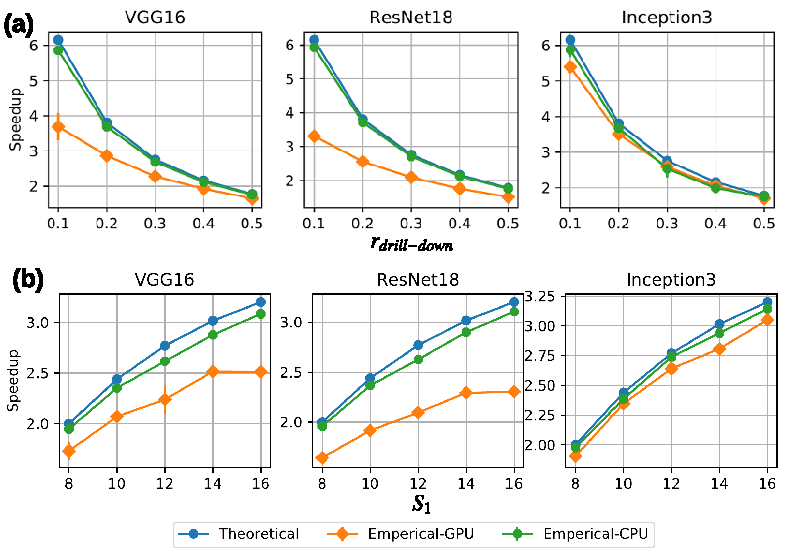
\includegraphics[width=\columnwidth]{images/5_2_3_GPU}
\caption{Theoretical versus empirical speedup for \textit{adaptive drill-down} with (a) varying drill-down ratios ($r_{drill-down}$) and (b) varying stage one stride $S_1$ values for different CNN models (Occlusion patch size = $16 \times 16$, stage two stride $S_2=4$, projective field threshold $\tau=1.0$).}
\label{fig:5_2_3_GPU}
\end{figure}

\vspace{2mm}
\noindent \textbf{Summary of Experimental Results.}